\section{Torque Study}\insertloftspace
\setcounter{figure}{0}\setcounter{table}{0}

\subsection{General principal}

As soon as we were able to create the first model, we were interested in the necessary motor torque. The objective was to determine the characteristics of each joint. Even if it was not the final robot, the different prototypes allowed us to have an estimation that we updated as soon as a choice was made. 

\bigbreak
In order to determine the necessary motors, we measured the following variables:
\begin{multicols}{3}
    \begin{itemize}[noitemsep]
        \item torque
        \item rotation speed
        \item power
    \end{itemize}
\end{multicols}

\bigbreak
\begin{figure}[ht]
    \centering
    \includegraphics[width=0.8\textwidth]{Images/Section06/sensing\_joint.png}
    \caption{Joint sensing block}
    \label{fig:SensingBlock}
\end{figure}
\FloatBarrier

\bigbreak
All these measurements were made in simulation with Matlab. In the simscape model, we can modify the linkage blocks to return the torque and speed. The Power is measured by multiplying the two. The units are not specified and depend on the units defined. In our case : 
\begin{multicols}{2}
    \begin{itemize}[noitemsep]
        \item length: m
        \item time: s
        \item mass: kg
        \item angle: rad
        \item force: N
        \item power: W
    \end{itemize}
\end{multicols}

We remind the relationship between torque, speed, and power: 
\begin{center}
    $P\hspace{0.3cm}=\hspace{0.3cm}CW$    
\end{center}

\bigbreak
To make these measurements, we built the following model: a block to send a trajectory, a block for inverse kinematics, and a block of simulation on which we come to carry out the measurements. It was important not to control the position of the links directly to avoid any discontinuity. Indeed, it is necessary that all the functions are derivable twice as a function of time to calculate the torque and the speed of rotation. This is why we make our robot follow a given trajectory.
\begin{figure}[ht]
    \centering
    \includegraphics[width=0.8\textwidth]{Images/Section06/motors\_analysis\_simulink.png}
    \caption{Joint analysis model}
    \label{fig:JointGlobalModel}
\end{figure}
\FloatBarrier

\begin{figure}[ht]
    \centering
    \includegraphics[width=0.8\textwidth]{Images/Section06/motors\_analysis\_robot.png}
    \caption{Joint analysis robot measure}
    \label{fig:JointRobotModel}
\end{figure}
\FloatBarrier

\bigbreak
We develop in the following sub-sections the results for each link. After having estimated the characteristics a margin of 30\% was taken. Our consultant explained to us that it was a security. 

\bigbreak
In reality, only the power delivered interested us to select the engines. Indeed, if an engine is able to provide a certain power, we must look at the tuple (torque, speed) allowing this power. If one of the two does not meet the necessary values, a gear can be added. Let's take a gear of speed $r$, $\omega'= r\omega$ and $C'= \frac{C}{r}$ or $P'= \omega'C'=r\omega\frac{C}{r} = \omega C = P$. The gear allows changing the torque and the speed without modifying the power. Therefore, a corresponding gear must exist.

\bigbreak
A static study was also conducted. We placed the robot in the "worst" configuration for each link and then we measured the torque required to maintain the robot in this position. The torques indicated on the motors' data sheet do not usually guarantee a static hold. To make sure that our motors are powerful enough, we multiplied this value by 3 to choose them. 

\bigbreak
The table below lists the characteristics required for each linkage as well as the estimates obtained on the first prototype. It is important to note that this one, although farther from reality, is still close. Moreover, the final values are all lower because we have reduced the mass of the robot. In order to anticipate the delivery time, we based ourselves on results obtained on intermediate prototypes. We can then validate this method. 

\begin{table}[ht]
    \centering
    \begin{tabular}{|p{1.5cm} | p{4cm} | p{4cm}|p{5cm} |} 
        \hline
        \textbf{Joint} & \textbf{Power/estimate (W)} & \textbf{Torque/estimate (N)}& \textbf{Angulare speed/estimate (rad/s)}\\ [0.3ex] 
        \hline\
        Pelvis & 0.2/1 & 0.2/4.2 & 0.9/0.23 \\ 
        \hline
        Shoulder & 1.8/4 & 5.4/9.8 & 0.77/0.4 \\ 
        \hline
        Elbow & 0.7/2.3 & 2.07/2.4 & 0.78/0.94 \\ 
        \hline
        Wrist & 0.23/0.4 & 0.38/1.1 & 0.94/0.35 \\ 
        \hline
    \end{tabular}
    \caption{Power, torque, and speed rotation needed per joint}
\end{table}
\FloatBarrier

\subsection{Static}

For the static study, we put the robot in the position that requires the most effort to hold it in place. It is thus in a horizontal position with its arm stretched out. This is indeed the position where the leverage is the most important for the shoulder, the elbow, and the wrist. In the static position, there is never any effort on the pelvis.
\begin{figure}[ht]
    \centering
    \includegraphics[width=0.6\textwidth]{Images/Section06/static\_torque\_position.png}
    \caption{Static position}
    \label{fig:StaticPosition}
\end{figure}
\FloatBarrier

\bigbreak
We obtain the following results. We have plotted in blue the measured value and in red the value that our motor must be able to provide to ensure that it will be able to maintain this position. The torques indicated on the data sheets are generally dynamic torques and not static. According to the advice given to us, we take three times the value obtained in static to be sure the motor will be able to give enough torque.
\begin{figure}[ht]
    \centering
    \includegraphics[width=0.8\textwidth]{Images/Section06/static\_torque.png}
    \caption{Static torque}
    \label{fig:StaticTorque}
\end{figure}
\FloatBarrier

\bigbreak
These values could have been calculated manually. ONSHAPE allows finding the mass and the position of the center of gravity for a given set of parts. Thus, by retrieving the mass and the distance between the center of gravity and the link, we could have calculated the torque by assimilating the set of selected parts to a point of mass $m$ at a distance $d$ from the link.
\begin{center}
    $C\hspace*{0.3cm}=\hspace*{0.3cm}m*g*d$
\end{center}
\begin{table}[ht]
    \centering
    \begin{tabular}{|p{1.5cm} | p{2cm} | p{2.5cm}| p{2.7cm} | p{2.7cm} |} 
        \hline
        \textbf{Joint} & \textbf{Mass (kg)} & \textbf{Distance (m)}& \textbf{Torque (N.m)}& \textbf{Matlab (N.m)}\\ [0.3ex] 
        \hline
        Shoulder & 0.852 & 0.222 & 1.8 & 1.8 \\ 
        \hline
        Elbow & 0.460 & 0.152 & 0.68 & 0.68 \\ 
        \hline
        Wrist & 0.165 & 0.78 & 0.13 & 0.13 \\ 
        \hline
    \end{tabular}
    \caption{Static torque}
\end{table}
\FloatBarrier

\bigbreak
It can be noted that the values calculated and measured via Matlab are approximately identical. This also allows us to validate our measurement model and to make sure that we can rely on the values found with the simulation to choose the motors.

\subsection{Joint movement}

For each of the links, we conjectured the most "difficult" trajectory to achieve. We then tested it as well as different trajectories to make sure that we were right. The duration was also chosen according to the amplitude of the movement in order to meet the speed criterion defined in the specifications. We present here only the trajectory having presented the highest values. A margin of 30 \% was then retained following the advice of our consultant to take into account the frictions as well as the possible differences between the simulation and the reality.

\subsubsection{Pelvis}

In the case of the pelvis, the motor needs the most power when the arm is stretched horizontally and rotates around the base. So we made the robot make a half circle in 2s to measure the torque, the power, and the rotation speed.
\begin{figure}[ht]
    \centering
    \includegraphics[width=0.6\textwidth]{Images/Section06/motors\_analysis\_pelvis\_trajectory1.png}
    \caption{Pelvis trajectory seen from top}
    \label{fig:PelvisTrajectory}
\end{figure}
\FloatBarrier

\bigbreak
As we can see on the graph below, in this case, the maximum power is $0.15W$. For this power, the torque is $0.16N.m$ and the rotation speed is $0.95rad.s^{-1}$. By adding 30\% we obtain a power of $0.2W$ and a torque of $0.21N.m$. The torque being superior to the one found to maintain the arm in static, finding a motor capable of delivering such power will be sufficient.
\begin{figure}[ht]
    \centering
    \includegraphics[width=0.7\textwidth]{Images/Section06/motors\_analysis\_pelvis1.png}
    \caption{Pelvis characteristics}
    \label{fig:PelvisCharacteristics}
\end{figure}
\FloatBarrier

\subsubsection{Shoulder}

In the case of the shoulder, the motor needs the most power when the arm starts stretched horizontally and rises only around this axis. So we made the robot make a quarter circle in 2s to measure the torque, the power, and the rotation speed.
\begin{figure}[ht]
    \centering
    \includegraphics[width=0.5\textwidth]{Images/Section06/motors\_analysis\_shoulder\_trajectory1.png}
    \caption{Shoulder trajectory seen from side}
    \label{fig:ShoulderTrajectory}
\end{figure}
\FloatBarrier

\bigbreak
As we can see on the graph below, in this case, the maximum power is $1.41W$. For this power, the torque is $1.83N.m$ and the rotation speed is $0.77rad.s^{-1}$. By adding 30\% we obtain a power of $1.83W$ and a torque of $2.34N.m$. The torque found is lower than the one needed to keep the robot static, so care must be taken to deliver both the power and the torque needed.
\begin{figure}[ht]
    \centering
    \includegraphics[width=0.7\textwidth]{Images/Section06/motors\_analysis\_shoulder1.png}
    \caption{Shoulder characteristics}
    \label{fig:ShoulderCharacteristics}
\end{figure}
\FloatBarrier

\subsubsection{Elbow}

In the case of the elbow, the motor needs the most power when the arm starts at 90 degrees at this link and rotates to a horizontal position. So we made the robot make a quarter circle in 2s to measure the torque, the power, and the rotation speed.

\begin{figure}[ht]
    \centering
    \includegraphics[width=0.5\textwidth]{Images/Section06/motors\_analysis\_elbow\_trajectory1.png}
    \caption{Elbow trajectory}
    \label{fig:ElbowTrajectory}
\end{figure}
\FloatBarrier

As we can see on the graph below, in this case, the maximum power is $0.51W$. For this power, the torque is $0.66N.m$ and the rotation speed is $0.77rad.s^{-1}$. By adding 30\% we obtain a power of $0.67W$ and a torque of $0.86N.m$. The torque found is lower than the one needed to keep the robot static, so care must be taken to deliver both the power and the torque needed.
\begin{figure}[ht]
    \centering
    \includegraphics[width=0.7\textwidth]{Images/Section06/motors\_analysis\_elbow1.png}
    \caption{Elbow characteristics}
    \label{fig:ElbowCharacteristics}
\end{figure}
\FloatBarrier

\subsubsection{Wrist}

In the case of the wrist, the motor needs the most power when the arm starts at 45 degrees at this link and rotates around. So we made the robot make a quarter circle in 2s to measure the torque, the power, and the rotation speed.

\begin{figure}[ht]
    \centering
    \includegraphics[width=0.5\textwidth]{Images/Section06/motors\_analysis\_wrist\_trajectory1.png}
    \caption{Wrist trajectory}
    \label{fig:WristTrajectory}
\end{figure}
\FloatBarrier

As we can see on the graph below, in this case, the maximum power is $0.18W$. For this power, the torque is $0.19N.m$ and the rotation speed is $0.94rad.s^{-1}$. By adding 30\% we obtain a power of $0.23W$ and a torque of $0.24N.m$. The torque found is lower than the one needed to keep the robot static, so care must be taken to deliver both the power and the torque needed.
\begin{figure}[ht]
    \centering
    \includegraphics[width=0.7\textwidth]{Images/Section06/motors\_analysis\_wrist1.png}
    \caption{Wrist characteristics}
    \label{fig:WristCharacteristics}
\end{figure}
\FloatBarrier

\subsection{Hardware choices}

Just as we presented the results on the final robot for the torque, we also continue here. So the gears we will calculate will not be the ones we have mounted on the robot because we had based ourselves on the intermediate model. To speed up the manufacturing of the robot, we decided to buy servo motors so that we don't have to do any electronics. Dynamixel \cite{Dynamixel} motors were thus recommended. First, because they are widely used in robotics and very reliable but also because a ROS package has already been created with many examples to integrate them very quickly into our software. We have only selected the motors provided by this company by respecting two criteria: a reasonable price and the necessary characteristics respected by adding a gear if necessary.

\begin{figure}[ht]
    \centering
    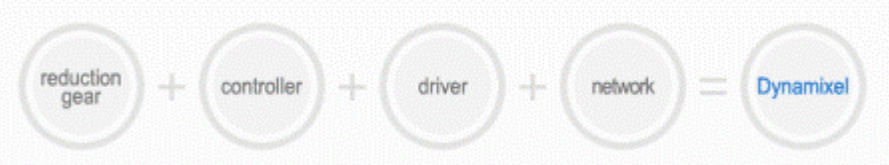
\includegraphics[width=0.8\textwidth]{Images/Section06/dynamixel.png}
    \caption{Dynamixel servomotor principle}
    \label{fig:DynamixelPrinciple}
\end{figure}
\FloatBarrier

\subsubsection{Pelvis}

In view of the different models available at dynamixel, we have selected the following engine: \textbf{dynamixel XL430-W250}. The following graph shows the performance of the motor. In particular, in black, the maximum torque that can be delivered according to the speed of rotation of the motor. By multiplying the two we obtain the maximum power.
\begin{figure}[ht]
    \centering
    \includegraphics[width=0.5\textwidth]{Images/Section06/pelvis\_motor\_specification.png}
    \caption{Pelvis motor performance}
    \label{fig:PelvisMotor}
\end{figure}
\FloatBarrier

\bigbreak
The necessary characteristics measured at the time as well as the one measured with the last version and the one of the engine are summarized below.
\begin{table}[ht]
    \centering
    \begin{tabular}{|p{1.5cm} | p{2cm} | p{2.5cm}| p{2.7cm} | p{2.7cm} |} 
        \hline
        \textbf{Joint}& \textbf{Power (W)} & \textbf{Torque (N.m)} & \textbf{Angular Speed (rad/s)} & \textbf{Static torque (N.m)}\\ [0.3ex]
        \hline
        previous need & 1 & 4.2 & 0.1 & 0 \\ 
        \hline
        actual need & 0.2 & 0.2 & 0.9 & 1.4 \\ 
        \hline
        motor & 0.65 & 0.73 & 0.9 & 1.5\\ 
        \hline
    \end{tabular}
    \caption{Pelvis motor specification}
\end{table}
\FloatBarrier
The motor is able to deliver directly the necessary dynamic and static values. No gearbox is really necessary. However, at the time we made the measurements, because of a more approximate model and our less good mastery of MATLAB, we had found much higher values. So we calculated that we needed a gear with a ratio of 1/7.

\subsubsection{Shoulder}

 We have selected the following engine: \textbf{dynamixel XM430-W350}. The following graph shows the performance of the motor. In particular, in black, the maximum torque that can be delivered according to the speed of rotation of the motor. By multiplying the two we obtain the maximum power.
\begin{figure}[ht]
    \centering
    \includegraphics[width=0.5\textwidth]{Images/Section06/shoulder\_motor\_performance.png}
    \caption{Shoulder motor performance}
    \label{fig:ShoulderMotor}
\end{figure}
\FloatBarrier

\bigbreak
The necessary characteristics measured at the time as well as the ones measured with the last version and the one of the engine are summarized below.
\begin{table}[ht]
    \centering
    \begin{tabular}{|p{1.5cm} | p{2cm} | p{2.5cm}| p{2.7cm} | p{2.7cm} |} 
        \hline
        \textbf{Joint}& \textbf{Power (W)} & \textbf{Torque (N.m)} & \textbf{Angular Speed (rad/s)} & \textbf{Static torque (N.m)}\\ [0.3ex]
        \hline
        previous need & 2.8 & 7.6 & 0.4 & 5.2 \\ 
        \hline
        actual need & 1.8 & 2.4 & 0.77 & 5.1 \\ 
        \hline
        motor & 2.3 & 2.87 & 0.83 & 4.1\\ 
        \hline
    \end{tabular}
    \caption{Shoulder motor specification}
\end{table}
\FloatBarrier
The motor is able to deliver directly the necessary dynamic values. However, the static torque is not sufficient and a gearbox will then be necessary with a ratio $r=\frac{4.1}{5.1}=1.3$. At the time we made the measurements, we had found higher values. So we calculated that we needed a gear with a ratio of 1/4.8.

\bigbreak
After mounting the robot, we measured the percentage of the maximum torque used by the motor to make the same trajectory. We realized that we are not even using 10\% of the maximum value. This confirms that the simulation results on the last prototype are much closer to reality and that we could replace the present gears.

\subsubsection{Elbow}


 We have selected the following engine: \textbf{dynamixel XC430-W150}. The following graph shows the performance of the motor. In particular, in black, the maximum torque that can be delivered according to the speed of rotation of the motor. By multiplying the two we obtain the maximum power.
\begin{figure}[ht]
    \centering
    \includegraphics[width=0.5\textwidth]{Images/Section06/elbow\_motor\_specification.png}
    \caption{Elbow motor performance}
    \label{fig:ElbowMotor}
\end{figure}
\FloatBarrier

\bigbreak
The necessary characteristics measured at the time as well as the ones measured with the last version and the one of the engine are summarized below.
\begin{table}[ht]
    \centering
    \begin{tabular}{|p{1.5cm} | p{2cm} | p{2.5cm}| p{2.7cm} | p{2.7cm} |} 
        \hline
        \textbf{Joint}& \textbf{Power (W)} & \textbf{Torque (N.m)} & \textbf{Angular Speed (rad/s)} & \textbf{Static torque (N.m)}\\ [0.3ex]
        \hline
        previous need & 2.26 & 2.4 & 1 & 1.86 \\ 
        \hline
        actual need & 0.7 & 0.86 & 0.78 & 2.07 \\ 
        \hline
        motor & 1.2 & 0.7 & 0.83 & 1.6\\ 
        \hline
    \end{tabular}
    \caption{Elbow motor specification}
\end{table}
\FloatBarrier
The motor is able to deliver directly the necessary dynamic power. However, the static and dynamic torques are not sufficient and a gearbox will then be necessary with a ratio $r=\frac{2.07}{1.6}=1.3$. The dynamic torque needs a ratio of $r=\frac{0.86}{0.7}=1.23$, a ratio of 1.3 is then perfect. At the time we made the measurements, we had found higher values. So we calculated that we needed a gear with a ratio of 1/5.

\bigbreak
After mounting the robot, we measured the percentage of the maximum torque used by the motor to make the same trajectory. We realized that we are not even using 20\% of the maximum value. This confirms that the simulation results on the last prototype are much closer to reality and that we could replace the present gears.

\subsubsection{Wrist}

In view of the different models available at dynamixel, we have selected the following engine: \textbf{dynamixel XL430-W250}. The following graph shows the performance of the motor. In particular, in black, the maximum torque that can be delivered according to the speed of rotation of the motor. By multiplying the two we obtain the maximum power.
\begin{figure}[ht]
    \centering
    \includegraphics[width=0.5\textwidth]{Images/Section06/pelvis\_motor\_specification.png}
    \caption{Wrist motor performance}
    \label{fig:WristMotor}
\end{figure}
\FloatBarrier

\bigbreak
The necessary characteristics measured at the time as well as the ones measured with the last version and the one of the engine are summarized below.
\begin{table}[ht]
    \centering
    \begin{tabular}{|p{1.5cm} | p{2cm} | p{2.5cm}| p{2.7cm} | p{2.7cm} |} 
        \hline
        \textbf{Joint}& \textbf{Power (W)} & \textbf{Torque (N.m)} & \textbf{Angular Speed (rad/s)} & \textbf{Static torque (N.m)}\\ [0.3ex]
        \hline
        previous need & 0.36 & 1.04 & 0.35 & 0 \\ 
        \hline
        actual need & 0.23 & 0.24 & 0.95 & 0.38 \\ 
        \hline
        motor & 0.65 & 0.73 & 0.9 & 1.5\\ 
        \hline
    \end{tabular}
    \caption{Wrist motor specification}
\end{table}
\FloatBarrier
The motor is able to deliver directly the necessary dynamic and static values. No gearbox is really necessary. However, at the time we made the measurements, because of a more approximate model and our less good mastery of MATLAB, we had found much higher values. So we calculated that we needed a gear with a ratio of 1/2.2.